%!TEX root = ../main.tex
%%%%%%%%%%%%%%%%%%%%%%%%%%%%%%%%%%
% Links:
%
% Difficulty:
% Companies: 
%%%%%%%%%%%%%%%%%%%%%%%%%%%%%%%%%%


%\begin{figure}
%	\centering
%	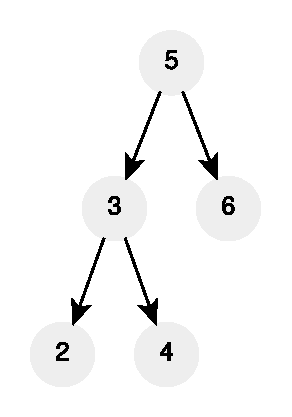
\includegraphics[width=\textwidth]{sources/merge_k_sorted_lists/images/example1}
%	\caption[Sample short cpation]{Sample Caption}.
%	\label{fig:merge_k_sorted_lists:example1}
%\end{figure}

\chapter{Merge $k$ sorted lists}
\label{ch:merge_k_sorted_lists}
\section*{Introduction}
The problem discussed in this chapter is quite interesting because it is rooted on the familiar  merge-sort algorithm\cite{wiki:mergesort} which is a divide and conquer algorithm that works by first splitting a list into smaller and smaller ones (see figure \ref{fig:merge_k_sorted_lists:example_mergesort}) and then sorts them separately and then it merges them a pair at the time preserving the sorting property (see figure \ref{fig:merge_k_sorted_lists:example_mergesort_1}). 
In this chapter we will focus on the merge phase and, in particular, we will try to find an efficient way to augment it so that we it will be capable of merging more than only a pair of sorted lists. 

Coming up with a brute-force solution for merging $k$ lists is not hard but the resulting end algorithm is rather inefficient. 
A faster and more efficient approach requires a bit more effort, and in the remainder of the chapter we will investigate a couple of different approaches that we can take to solve this problem efficiently.
In particular, we will have a look at the brute-force solution (in Section \ref{merge_k_sorted_lists:sec:bruteforce}) and then at two approaches we can take to lower the overall time and space complexity (in Section \ref{merge_k_sorted_lists:sec:priorityqueue} and \ref{merge_k_sorted_lists:sec:divideetimpera}).


\begin{figure}
	\centering
	\begin{subfigure}[t]{0.80\textwidth}
		\caption[]{First phase of the merge-sort where the a list is recursively split into smaller ones (~ half the original length) until we are left with lists of size $1$}.
		\label{fig:merge_k_sorted_lists:example_mergesort}
		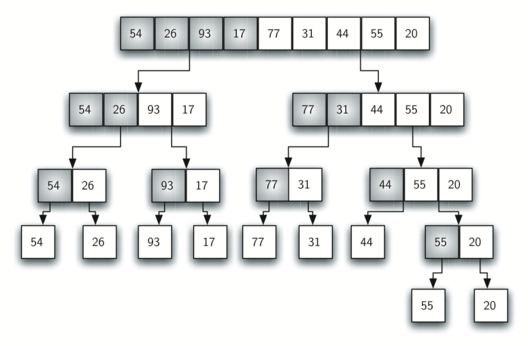
\includegraphics[width=\textwidth]{sources/merge_k_sorted_lists/images/mergesort_example}
	 \end{subfigure}
	\hfill
	\begin{subfigure}[t]{0.80\textwidth}
		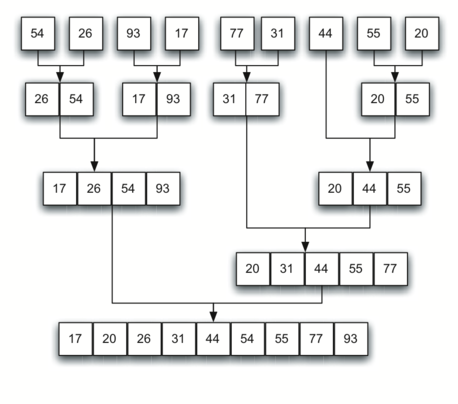
\includegraphics[width=\textwidth]{sources/merge_k_sorted_lists/images/mergesort_example_1}
		\caption[]{Second phase of the merge-sort where the split lists are recursively merged preserving the sorting property.}.
		\label{fig:merge_k_sorted_lists:example_mergesort_1}
	 \end{subfigure}
\end{figure}

\section{Problem statement}
\begin{exercise}
\label{example:merge_k_sorted_lists:exercice1}
Write a function that, given $k$ lists that are sorted in ascending order, merges them into a new sorted list.

	%example1
	\begin{example}
		\label{example:merge_k_sorted_lists:example1}
		\hfill \\ 
		Given \inline{L=[[1,4,5],[1,3,4],[2,6]} the function returns \inline{[1,1,2,3,4,4,5,6]}
	\end{example}

	%example2
	\begin{example}
		\label{example:merge_k_sorted_lists:example2}
		\hfill \\ Given \inline{L=[[1,2,3],[4,5,6],[7,8,9]} the function returns \inline{[1,2,3,4,5,6,7,8,9]}
	\end{example}

	\begin{example}
		\hfill \\ Given \inline{L=[[7,8,9],[4,5,6],[1,2,3]} the function returns \inline{[1,2,3,4,5,6,7,8,9]}
	
	\label{ex:merge_k_sorted_lists:example3}
	\end{example}

\end{exercise}

\section{Clarification Questions}

\begin{QandA}
	\item 
	\begin{answered}
		\textit{}
	\end{answered}
	
\end{QandA}

\section{Discussion}
\label{merge_k_sorted_lists:sec:discussion}


\subsection{Brute-force}
\label{merge_k_sorted_lists:sec:bruteforce}

	\lstinputlisting[language=c++, caption={Brute-force solution.},label=list:merge_k_sorted_lists_bruteforce]{sources/merge_k_sorted_lists/merge_k_sorted_lists_solution1.cpp}


\subsection{Priority-queue approach}
\label{merge_k_sorted_lists:sec:priorityqueue}

\lstinputlisting[language=c++, caption={Priority-queue-based solution.},label=list:merge_k_sorted_lists_prioqueue]{sources/merge_k_sorted_lists/merge_k_sorted_lists_solution2.cpp}

\subsection{Divide et impera}
\label{merge_k_sorted_lists:sec:divideetimpera}

